\section{Consuntivo di periodo}
		In questa sezione verranno riportati il consuntivo per le varie fasi di lavoro, considerando le ore sostenute da ogni componente per ruolo. Il bilancio potrà essere:
		\begin{itemize}
			\item \textbf{positivo:} se sono state necessarie meno ore rispetto a quelle preventivate;	 
			\item \textbf{paritario:} se le ore preventivate rispettano quelle effettive;	 
			\item \textbf{negativo:} se sono state necessarie più ore rispetto a quelle preventivate.
		\end{itemize}
	\subsection{Fase di Analisi}
		Le ore di lavoro svolto in questo periodo sono di solo investimento e destinate all'apprendimento personale. Di conseguenza queste ore non sono rendicontate. 
		\subsubsection{Prospetto orario}
			Nella tabella in seguito viene illustrato il cambiamento nel numero d'ore di ogni persona, per ogni ruolo ricoperto:
			
			\rowcolors{2}{white}{lightest-grayest}
			\begin{longtable}{|c|c|c|c|c|c|c|c}
				\hline
				\rowcolor{lighter-grayer}
				\textbf{Nome} & \textbf{Re} & \textbf{Am} & \textbf{An} & \textbf{Pg}  & \textbf{Pr}   & \textbf{Ve} & \textbf{Totale} \\
				\hline
				\endfirsthead
				
				\hline
				Giuseppe Vito Bitetti 		& 0 & 8(-1) & 10(+1) & 0 & 0 & 12 & 30\\
				\hline
				\hline
				Lorenzo Dei Negri			 & 6(-2) & 0 & 14(+1) & 0 & 0 & 10(+1) & 30\\
				\hline
				\hline
				Nicolò Frison 					& 0 & 8(-2) & 9(+1) & 0 & 0 & 13(+1) & 30\\
				\hline
				\hline
				Fouad Mouad 				& 0 & 7 & 11 & 0 & 0 & 12 & 30\\
				\hline
				\hline
				Mariano Sciacco 			& 8 & 0 & 12 & 0 & 0 & 10 & 30\\
				\hline
				\hline
				Alessandro Tommasin    & 9(-2) & 0 & 12(+2) & 0 & 0 & 9 & 30\\
				\hline
				\hline
				Giovanni Vidotto 			& 0 & 6(-1) & 9(+1) & 0 & 0 & 15 & 30\\
				\hline 
				\caption{Tabella contenente il prospetto orario preventivato per la fase di analisi}
			\end{longtable}
			\pagebreak	
			
			La tabella può essere riassunta nel seguente istogramma:
			
			\begin{figure}[H]
				\centering
				\includegraphics[width=0.8\linewidth]{./images/analisiCons1.png}
				\caption{Grafico consuntivo ore/ruolo componenti nella fase di Analisi}
				\label{fig:consuntivo grafico suddivione ruoli fase Analisi}
			\end{figure}
			
		\subsubsection{Prospetto economico}
			In base al prospetto orario, quello economico sarà il seguente: 
			
			\rowcolors{2}{white}{lightest-grayest}
			\begin{longtable}{|c|c|c|c|c|c|c|c}
				\hline
				\rowcolor{lighter-grayer}
				\textbf{Ruolo} & \textbf{Ore} & \textbf{Costo in €} \\
				\hline
				\endfirsthead
				
				\hline
				Responsabile & 23(-4) & 690,00 (-120,00)\\
				\hline
				\hline
				Amministratore & 29(-4) & 580,00 (-80,00)\\
				\hline
				\hline
				Analista & 77(+6) & 1.925,00(+150,00)\\
				\hline
				\hline
				Progettista & - & -\\
				\hline
				\hline
				Programmatore & - & -\\
				\hline
				\hline
				Verificatore & 81(+2) & 1.215,00(+30,00)\\
				\hline
				\textbf{Totale} & 210 & 4.410,00(-20,00)\\
				\hline
				\caption{Tabella contenente il prospetto economico in riferimento al prospetto orario nella tabella 17}
			\end{longtable}
			\pagebreak
			
			La tabella può essere riassunta nel seguente areogramma:
			\begin{figure}[H]
				\centering
				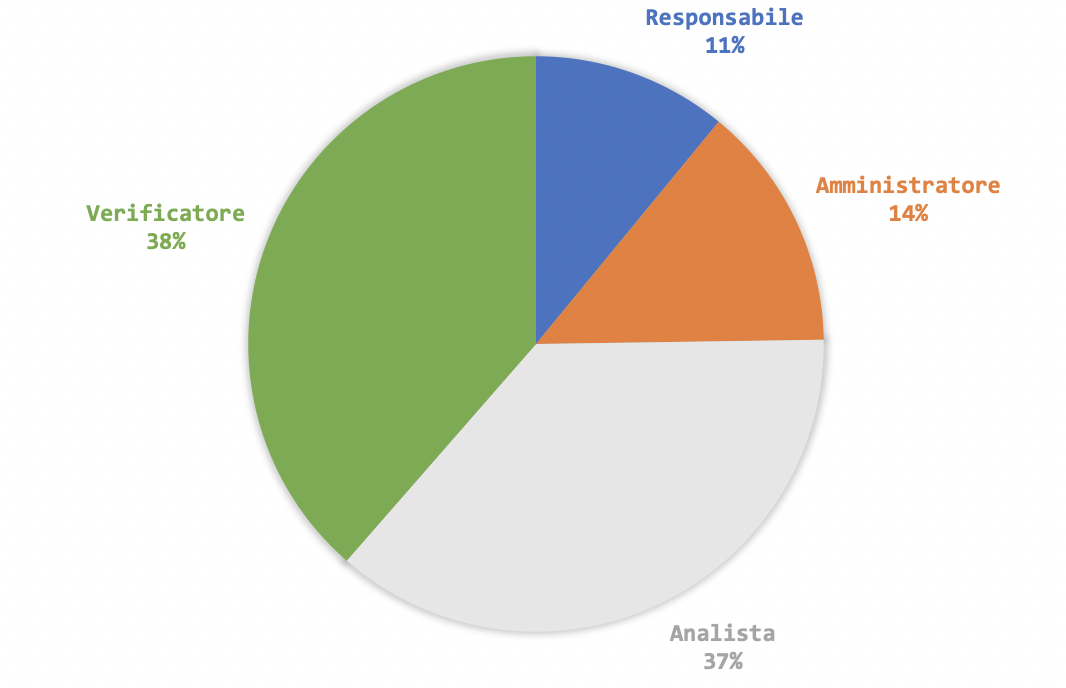
\includegraphics[width=0.8\linewidth]{./images/analisiCons2.png}
				\caption{Grafico percentuale ore/ruolo nella fase di Analisi dei requisiti}
				\label{fig:grafico costi ruolo fase Analisi}
			\end{figure}
		
		

		\subsection{Fase di Consolidamento dei Requisiti}
		Le ore di lavoro svolte in questo periodo sono volte alla preparazione della presentazione e alla revisione dei requisiti individuati. 
		\subsubsection{Prospetto orario}
			Nella tabella in seguito viene illustrato il cambiamento nel numero d'ore di ogni persona, per ogni ruolo ricoperto:
			
			\rowcolors{2}{white}{lightest-grayest}
			\begin{longtable}{|c|c|c|c|c|c|c|c}
				\hline
				\rowcolor{lighter-grayer}
				\textbf{Nome} & \textbf{Re} & \textbf{Am} & \textbf{An} & \textbf{Pg}  & \textbf{Pr}   & \textbf{Ve} & \textbf{Totale} \\
				\hline
				\endfirsthead
				
				\hline
				Giuseppe Vito Bitetti & 0 & 0 & 5 & 0 & 0 & 0 & 5\\
				\hline
				\hline
				Lorenzo Dei Negri & 0 & 5 & 0 & 0 & 0 & 0 & 5\\
				\hline
				\hline
				Nicolò Frison & 0 & 0 & 0 & 0 & 0 & 5 & 5\\
				\hline
				\hline
				Fouad Mouad & 2 (-1) & 0 & 0 (+1) & 0 & 0 & 3 & 5\\
				\hline
				\hline
				Mariano Sciacco & 0 & 0 & 3 & 0 & 0 & 2 & 5\\
				\hline
				\hline
				Alessandro Tommasin & 0 & 0 & 4 (+1) & 0 & 0 & 1 (-1) & 5\\
				\hline
				\hline
				Giovanni Vidotto & 2 & 0 & 0 & 0 & 0 & 3 & 5\\
				\hline 
				\textbf{Totale} & 4 (-1) &  5 & 12 (+2) & 0 & 0 & 14 (-1) & 35\\
				\hline
				\caption{Tabella contenente il prospetto orario preventivato per la fase di Consolidamento dei Requisiti}
			\end{longtable}
			\pagebreak	
			
			La tabella può essere riassunta nel seguente istogramma:
			
			\begin{figure}[H]
				\centering
				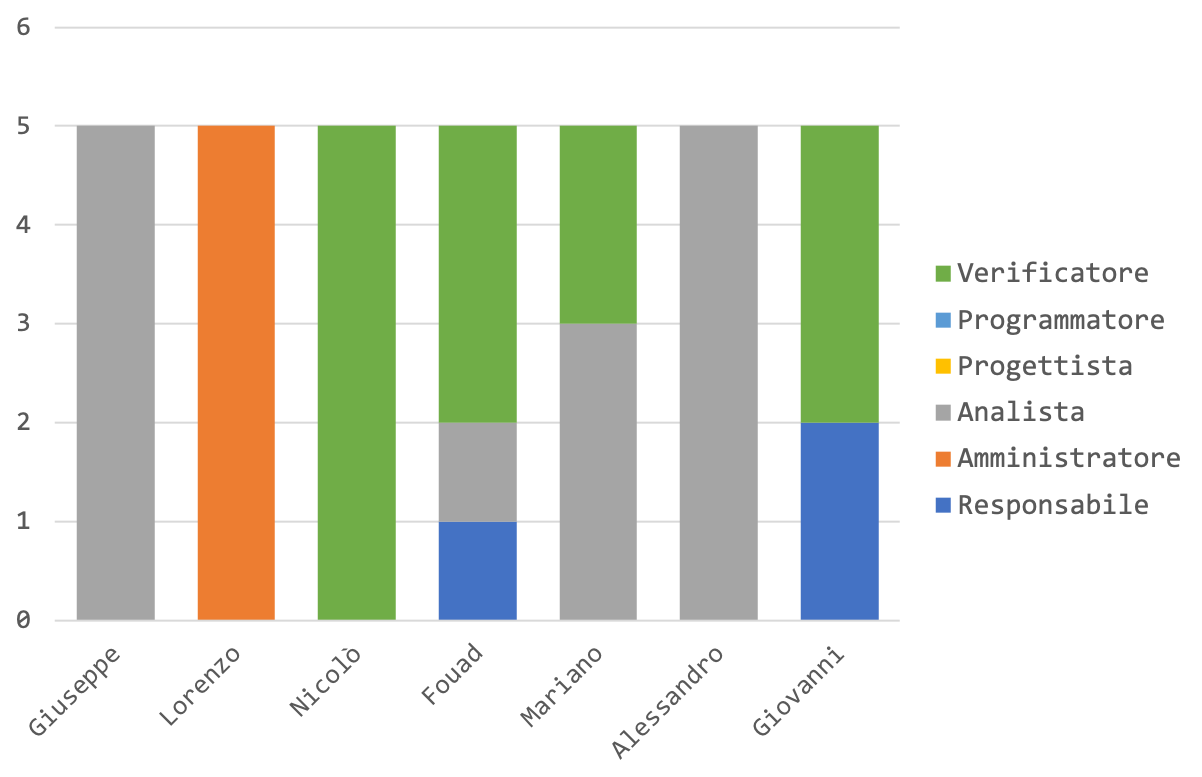
\includegraphics[width=0.8\linewidth]{./images/ConsReqCons.png}
				\caption{Grafico consuntivo ore/ruolo componenti della fase di Consolidamento dei Requisiti}
				\label{fig:consuntivo grafico suddivione ruoli fase di Consolidamento dei Requisiti}
			\end{figure}
			
		\subsubsection{Prospetto economico}
			In base al prospetto orario, quello economico sarà il seguente: 
			
			\rowcolors{2}{white}{lightest-grayest}
			\begin{longtable}{|c|c|c|c|c|c|c|c}
				\hline
				\rowcolor{lighter-grayer}
				\textbf{Ruolo} & \textbf{Ore} & \textbf{Costo in €} \\
				\hline
				\endfirsthead
				
				\hline
				Responsabile & 4(-1) & 120,00 (-30,00)\\
				\hline
				\hline
				Amministratore & 5 & 100,00\\
				\hline
				\hline
				Analista & 12(+2) & 300,00(+50,00)\\
				\hline
				\hline
				Progettista & - & -\\
				\hline
				\hline
				Programmatore & -  & -\\
				\hline
				\hline
				Verificatore & 14(-1) & 210,00(-15,00)\\
				\hline
				\textbf{Totale} & 35 & 730,00(+5,00)\\
				\hline
				\caption{Tabella contenente il prospetto economico in riferimento al prospetto orario nella tabella 19}
			\end{longtable}
			\pagebreak
			
			La tabella può essere riassunta nel seguente areogramma:
			\begin{figure}[H]
				\centering
				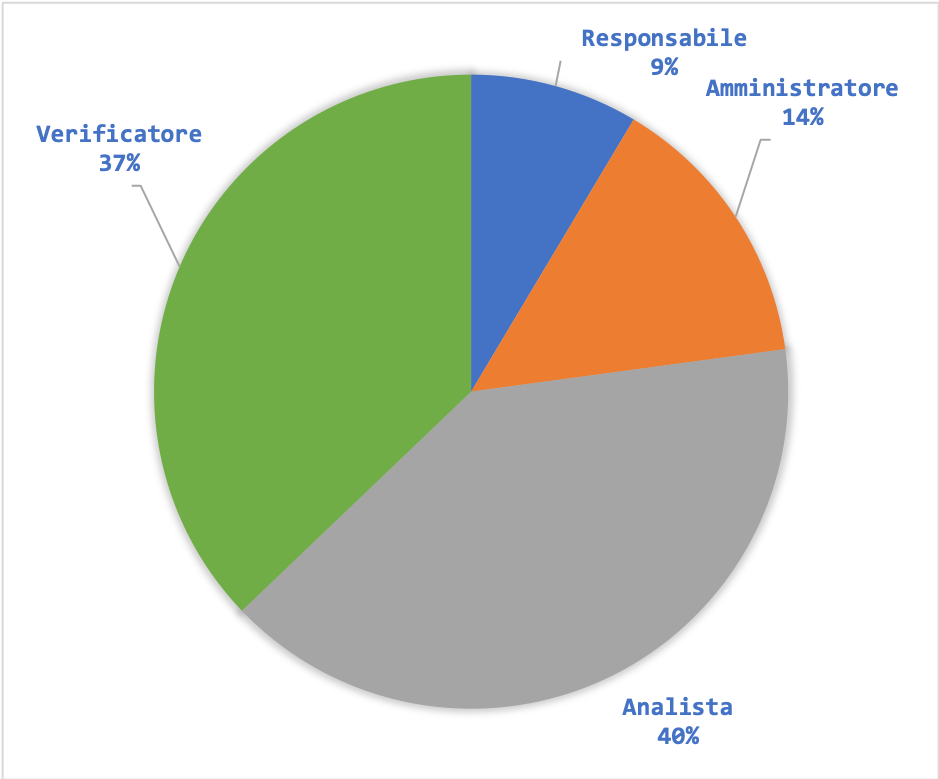
\includegraphics[width=0.8\linewidth]{./images/ConsReqCons2.png}
				\caption{Grafico percentuale ore/ruolo nella fase di Consolidamento dei Requisiti}
				\label{fig:grafico costi ruolo fase di Consolidamento dei Requisiti}
			\end{figure}
		
		\subsubsection*{Conclusioni }
			In questa fase il gruppo ha investito il numero di ore che erano state preventivate. È stato necessario però svolgere alcuni cambiamenti nella suddivisione oraria per ruolo, in particolare:
			\begin{itemize}
				\item \textbf{Responsabile:} sono state impiegate meno ore rispetto a quelle preventivate in quanto nella pianificazione del lavoro e nella stesura del Piano di Progetto sono state riscontrate meno difficoltà del previsto;	 
				\item \textbf{Amministratore:} dal momento che i software per la gestione del progetto sono stati individuati e configurati fin da subito e che i documenti sono stati ben strutturati in poco tempo, anche in questo caso sono state impiegate meno ore rispetto a quelle preventivate;	 
				\item \textbf{Analista:} per questo ruolo è stato necessario spendere qualche ora in più in quanto alcuni requisiti, per una corretta comprensione, hanno richiesto una delucidazione esterna con i proponenti del progetto, avvenuta con alcune difficoltà di comunicazione;
				\item \textbf{Verificatore:} poiché alcuni requisiti sono stati individuati tardivamente e di conseguenza per l'aggiunta di contenuti nel documento di Analisi dei Requisiti è stato necessario usufruire di qualche ora in più per controllare nuovamente il documento;
			\end{itemize}
			Alla luce dei cambiamenti effettuati il risultato è che il gruppo ha risparmiato 15,00 € investendo le stesse ore preventivate.

			

		\subsection{Fase di Progettazione della \textit{technology baseline}}
		Le ore di lavoro svolte in questo periodo sono volte alla progettazione della \textit{technology baseline} e alla realizzazione della \glock{proof of concept}. 
		\subsubsection{Prospetto orario}
			Nella tabella in seguito viene illustrato il cambiamento nel numero d'ore di ogni persona, per ogni ruolo ricoperto:
			
			\rowcolors{2}{white}{lightest-grayest}
			\begin{longtable}{|c|c|c|c|c|c|c|c}
				\hline
				\rowcolor{lighter-grayer}
				\textbf{Nome} & \textbf{Re} & \textbf{Am} & \textbf{An} & \textbf{Pg}  & \textbf{Pr}   & \textbf{Ve} & \textbf{Totale} \\
				\hline
				\endfirsthead
				\hline
				Giuseppe Vito Bitetti & 3 & 0 & 7 & 0 & 0 & 3 & 13\\
				\hline
				\hline
				Lorenzo Dei Negri & 0 & 5 & 1 & 5 & 0 & 2 & 13\\
				\hline
				\hline
				Nicolò Frison & 0 & 3 & 5 & 5 & 0 & 0 & 13\\
				\hline
				\hline
				Fouad Mouad & 0 & 4 & 3 & 2 & 0 & 4 & 13 \\
				\hline
				\hline
				Mariano Sciacco & 3 & 0 & 1 & 9 & 0 & 0 & 13\\
				\hline
				\hline
				Alessandro Tommasin & 0 & 4 & 6 & 0 & 0 & 3 & 13\\
				\hline
				\hline
				Giovanni Vidotto & 2 & 0 & 5 & 2 & 0 & 4 & 13\\
				\hline 
				\textbf{Totale} & 8 &  16 & 28 & 23 & 0 & 16 & 91 \\
				\hline
				
				\caption{Tabella contenente il prospetto orario preventivato per la fase di Progettazione della \textit{technology baseline}}
			\end{longtable}
			\pagebreak	
			
			La tabella può essere riassunta nel seguente istogramma:
			
			%\begin{figure}[H]
			%	\centering
			%	\includegraphics[width=0.8\linewidth]{./images/.png}
			%	\caption{Grafico consuntivo ore/ruolo componenti della fase di Progettazione della technology baseline}
			%	\label{fig:consuntivo grafico suddivione ruoli fase di Progettazione della technology baseline}
			%\end{figure}
			
		\subsubsection{Prospetto economico}
			In base al prospetto orario, quello economico sarà il seguente: 
			
			\rowcolors{2}{white}{lightest-grayest}
			\begin{longtable}{|c|c|c|c|c|c|c|c}
				\hline
				\rowcolor{lighter-grayer}
				\textbf{Ruolo} & \textbf{Ore} & \textbf{Costo in €} \\
				\hline
				\endfirsthead
				\hline
			Responsabile 	    & 8 & 240,00\\
			\hline 
			\hline
			Amministratore	  & 16 & 320,00\\
			\hline
			\hline
			Analista 				& 28 & 700,00\\
			\hline
			\hline
			Progettista 		  & 23 & 506,00\\
			\hline
			\hline
			Programmatore 	 & 0 & 0,00\\
			\hline
			\hline
			Verificatore 		  & 16 & 240,00\\
			\hline
			\textbf{Totale} 	& 91 & 2006,00\\
			\hline
				
				\caption{Tabella contenente il prospetto economico in riferimento al prospetto orario nella tabella 21}
			\end{longtable}
			\pagebreak
			
			La tabella può essere riassunta nel seguente areogramma:
			%\begin{figure}[H]
			%	\centering
			%	\includegraphics[width=0.8\linewidth]{./images/.png}
			%	\caption{Grafico percentuale ore/ruolo nella fase di Progettazione della technology baseline}
			%	\label{fig:grafico costi ruolo fase Progettazione della technology baseline}
			%\end{figure}
				
		
		\subsection{I Incremento}
		Le ore di lavoro svolte in questo periodo sono volte alla configurazione dei container e dell'immagine Docker di Kafka. 
		\subsubsection{Prospetto orario}
			Nella tabella in seguito viene illustrato il cambiamento nel numero d'ore di ogni persona, per ogni ruolo ricoperto:
			
			\rowcolors{2}{white}{lightest-grayest}
			\begin{longtable}{|c|c|c|c|c|c|c|c}
				\hline
				\rowcolor{lighter-grayer}
				\textbf{Nome} & \textbf{Re} & \textbf{Am} & \textbf{An} & \textbf{Pg}  & \textbf{Pr}   & \textbf{Ve} & \textbf{Totale} \\
				\hline
				\endfirsthead
				\hline
				Giuseppe Vito Bitetti & 0 & 0 & 3 & 0 & 2 & 0 & 5\\
				\hline
				\hline
				Lorenzo Dei Negri & 0 & 0 & 0 & 2 & 0 & 3 & 5\\
				\hline
				\hline
				Nicolò Frison & 0 & 3 & 0 & 0 & 0 & 2 & 5\\
				\hline
				\hline
				Fouad Mouad & 3 & 0 & 2 & 0 & 0 & 0 & 5\\
				\hline
				\hline
				Mariano Sciacco & 0 & 0 & 0 & 3 & 2 & 0 & 5\\
				\hline
				\hline
				Alessandro Tommasin & 0 & 2 & 0 & 3 & 0 & 0 & 5\\
				\hline
				\hline
				Giovanni Vidotto & 2 & 0 & 0 & 0 & 4 & 1 & 5\\
				\hline 
				\textbf{Totale} & 3 &  5 & 5 & 8 & 8 & 6 & 35\\
				\hline 
				
				\caption{Tabella contenente il prospetto orario preventivato per il I incremento}
			\end{longtable}
			\pagebreak	
			
			La tabella può essere riassunta nel seguente istogramma:
			
			%\begin{figure}[H]
			%	\centering
			%	\includegraphics[width=0.8\linewidth]{./images/.png}
			%	\caption{Grafico consuntivo ore/ruolo componenti del I incremento}
			%	\label{fig:consuntivo grafico suddivione ruoli I incremento}
			%\end{figure}
			
		\subsubsection{Prospetto economico}
			In base al prospetto orario, quello economico sarà il seguente: 
			
			\rowcolors{2}{white}{lightest-grayest}
			\begin{longtable}{|c|c|c|c|c|c|c|c}
				\hline
				\rowcolor{lighter-grayer}
				\textbf{Ruolo} & \textbf{Ore} & \textbf{Costo in €} \\
				\hline
				\endfirsthead
				\hline
			Responsabile 	    & 3 & 90,00\\
			\hline 
			\hline
			Amministratore	  & 5 & 100,00\\
			\hline
			\hline
			Analista 				& 5 & 125,00\\
			\hline
			\hline
			Progettista 		  & 8 & 176,00\\
			\hline
			\hline
			Programmatore 	 & 8 & 120,00\\
			\hline
			\hline
			Verificatore 		  & 6 & 90,00\\
			\hline
			\textbf{Totale} 	& 35 & 701,00\\
			\hline
				
				\caption{Tabella contenente il prospetto economico in riferimento al prospetto orario nella tabella 23}
			\end{longtable}
			\pagebreak
			
			La tabella può essere riassunta nel seguente areogramma:
			%\begin{figure}[H]
			%	\centering
			%	\includegraphics[width=0.8\linewidth]{./images/.png}
			%	\caption{Grafico percentuale ore/ruolo nel I incremento}
			%	\label{fig:grafico costi ruolo I incremento}
			%\end{figure}
		

		\subsection{II Incremento}
		Le ore di lavoro svolte in questo periodo sono volte alla creazione della struttura base del gateway ed alla decisione della struttura JSON dei dati da inviare a Kafka. Verrà inoltre implementato un primo protocollo di comunicazione.
		\subsubsection{Prospetto orario}
			Nella tabella in seguito viene illustrato il cambiamento nel numero d'ore di ogni persona, per ogni ruolo ricoperto:
			
			\rowcolors{2}{white}{lightest-grayest}
			\begin{longtable}{|c|c|c|c|c|c|c|c}
				\hline
				\rowcolor{lighter-grayer}
				\textbf{Nome} & \textbf{Re} & \textbf{Am} & \textbf{An} & \textbf{Pg}  & \textbf{Pr}   & \textbf{Ve} & \textbf{Totale} \\
				\hline
				\endfirsthead
				\hline
				Giuseppe Vito Bitetti & 0 & 0 & 0 & 3 & 0 & 3 & 6\\
				\hline
				\hline
				Lorenzo Dei Negri & 0 & 0 & 0 & 0 & 3 & 3 & 6 \\
				\hline
				\hline
				Nicolò Frison & 2 & 0 & 0 & 0 & 4 & 0 & 6 \\
				\hline
				\hline
				Fouad Mouad & 0 & 4 & 2 & 0 & 0 & 0 & 6 \\
				\hline
				\hline
				Mariano Sciacco & 0 & 0 & 0 & 3 & 0 & 3 & 6 \\
				\hline
				\hline
				Alessandro Tommasin & 2 & 0 & 0 & 0 & 4 & 0 & 6 \\
				\hline
				\hline
				Giovanni Vidotto & 0 & 2 & 0 & 4 & 0 & 0 & 6\\
				\hline 
				\textbf{Totale} & 4 &  6 & 2 & 10 & 11 & 9 & 42\\
				\hline 
				
				\caption{Tabella contenente il prospetto orario preventivato per il II incremento}
			\end{longtable}
			\pagebreak	
			
			La tabella può essere riassunta nel seguente istogramma:
			
			%\begin{figure}[H]
			%	\centering
			%	\includegraphics[width=0.8\linewidth]{./images/.png}
			%	\caption{Grafico consuntivo ore/ruolo componenti del II incremento}
			%	\label{fig:consuntivo grafico suddivione ruoli II incremento}
			%\end{figure}
			
		\subsubsection{Prospetto economico}
			In base al prospetto orario, quello economico sarà il seguente: 
			
			\rowcolors{2}{white}{lightest-grayest}
			\begin{longtable}{|c|c|c|c|c|c|c|c}
				\hline
				\rowcolor{lighter-grayer}
				\textbf{Ruolo} & \textbf{Ore} & \textbf{Costo in €} \\
				\hline
				\endfirsthead
				\hline
			Responsabile 	    & 4 & 120,00\\
			\hline 
			\hline
			Amministratore	  & 6 & 120,00\\
			\hline
			\hline
			Analista 				& 2 & 50,00\\
			\hline
			\hline
			Progettista 		  & 10 & 220,00\\
			\hline
			\hline
			Programmatore 	 & 11 & 165,00\\
			\hline
			\hline
			Verificatore 		  & 9 & 135,00\\
			\hline
			\textbf{Totale} 	& 42 & 810,00\\
			\hline
				
				\caption{Tabella contenente il prospetto economico in riferimento al prospetto orario nella tabella 25}
			\end{longtable}
			\pagebreak
			
			La tabella può essere riassunta nel seguente areogramma:
			%\begin{figure}[H]
			%	\centering
			%	\includegraphics[width=0.8\linewidth]{./images/.png}
			%	\caption{Grafico percentuale ore/ruolo nel II incremento}
			%	\label{fig:grafico costi ruolo II incremento}
			%\end{figure}

%%%%%%%%%%%%%%%%%%%%%%%%%%%%%%%%%%%%%%%%%%%%%%%%%%%%%%%%%%%%%%%%%%%%%%%%%%%%%%%%%%%%%%%%%%%%%%%%%%%%%%%%%%%%%%%%%%
		
		\subsection{III Incremento}
		Le ore di lavoro svolte in questo periodo sono volte alla progettazione dell'interfaccia delle API ed all'implementazione delle operazioni di lettura dei dati tramite le API.
		\subsubsection{Prospetto orario}
			Nella tabella in seguito viene illustrato il cambiamento nel numero d'ore di ogni persona, per ogni ruolo ricoperto:
			
			\rowcolors{2}{white}{lightest-grayest}
			\begin{longtable}{|c|c|c|c|c|c|c|c}
				\hline
				\rowcolor{lighter-grayer}
				\textbf{Nome} & \textbf{Re} & \textbf{Am} & \textbf{An} & \textbf{Pg}  & \textbf{Pr}   & \textbf{Ve} & \textbf{Totale} \\
				\hline
				\endfirsthead
				\hline
				Giuseppe Vito Bitetti & 0 & 0 & 0 & 0 & 3 & 3 & 6\\
				\hline
				\hline
				Lorenzo Dei Negri & 0 & 0 & 0 & 3 & 0 & 3 & 6\\
				\hline
				\hline
				Nicolò Frison & 1 & 0 & 0 & 2 & 0 & 3 & 6 \\
				\hline
				\hline
				Fouad Mouad & 0 & 0 & 0 & 3 & 3 & 0 & 6\\
				\hline
				\hline
				Mariano Sciacco & 0 & 3 & 0 & 0 & 3 & 0 & 6 \\
				\hline
				\hline
				Alessandro Tommasin & 2 & 0 & 0 & 2 & 2 & 0 & 6\\
				\hline
				\hline
				Giovanni Vidotto & 0 & 0 & 0 & 2 & 0 & 4 & 6 \\
				\hline 
				\textbf{Totale} & 3 &  3 & 0 & 12 & 1 & 13 & 42\\
				\hline 
				
				\caption{Tabella contenente il prospetto orario preventivato per il III incremento}
			\end{longtable}
			\pagebreak	
			
			La tabella può essere riassunta nel seguente istogramma:
			
			%\begin{figure}[H]
			%	\centering
			%	\includegraphics[width=0.8\linewidth]{./images/.png}
			%	\caption{Grafico consuntivo ore/ruolo componenti del III incremento}
			%	\label{fig:consuntivo grafico suddivione ruoli III incremento}
			%\end{figure}
			
		\subsubsection{Prospetto economico}
			In base al prospetto orario, quello economico sarà il seguente: 
			
			\rowcolors{2}{white}{lightest-grayest}
			\begin{longtable}{|c|c|c|c|c|c|c|c}
				\hline
				\rowcolor{lighter-grayer}
				\textbf{Ruolo} & \textbf{Ore} & \textbf{Costo in €} \\
				\hline
				\endfirsthead
				%Incollare tabella preventivo prospetto economico 
				
				\caption{Tabella contenente il prospetto economico in riferimento al prospetto orario nella tabella 27}
			\end{longtable}
			\pagebreak
			
			La tabella può essere riassunta nel seguente areogramma:
			%\begin{figure}[H]
			%	\centering
			%	\includegraphics[width=0.8\linewidth]{./images/.png}
			%	\caption{Grafico percentuale ore/ruolo nel III incremento}
			%	\label{fig:grafico costi ruolo III incremento}
			%\end{figure}

		%%%%%%%%%%%%%%%%%%%%%%%%%%%%%%%%%%%%%%%%%%%%%%%%%%%%%%%%%%%%%%%%%%%%%%%%%%%%%%%%%%%%%%%%%%%%%%%%%%%%%%%%%%%%%%%%%%
		
		\subsection{IV Incremento}
		Le ore di lavoro svolte in questo periodo sono volte alla configurazione di base della Webapp e reperimento dati dalle \glock{API}.
		\subsubsection{Prospetto orario}
			Nella tabella in seguito viene illustrato il cambiamento nel numero d'ore di ogni persona, per ogni ruolo ricoperto:
			
			\rowcolors{2}{white}{lightest-grayest}
			\begin{longtable}{|c|c|c|c|c|c|c|c}
				\hline
				\rowcolor{lighter-grayer}
				\textbf{Nome} & \textbf{Re} & \textbf{Am} & \textbf{An} & \textbf{Pg}  & \textbf{Pr}   & \textbf{Ve} & \textbf{Totale} \\
				\hline
				\endfirsthead
				\hline
				Giuseppe Vito Bitetti & 2 & 0 & 0 & 0 & 4 & 0 & 6\\
				\hline
				\hline
				Lorenzo Dei Negri & 2 & 0 & 2 & 2 & 0 & 0 & 6\\
				\hline
				\hline
				Nicolò Frison & 0 & 0 & 0 & 2 & 4 & 0 & 6\\
				\hline
				\hline
				Fouad Mouad & 0 & 3 & 0 & 0 & 0 & 3 & 6\\
				\hline
				\hline
				Mariano Sciacco & 3 & 0 & 0 & 0 & 3 & 0 & 6\\
				\hline
				\hline
				Alessandro Tommasin & 0 & 0 & 2 & 0 & 0 & 4 & 6\\
				\hline
				\hline
				Giovanni Vidotto & 0 & 0 & 0 & 5 & 0 & 1 & 6\\
				\hline 
				\textbf{Totale} & 7 &  3 & 4 & 9 & 11 & 8 & 42 \\
				\hline 
				
				\caption{Tabella contenente il prospetto orario preventivato per il IV incremento}
			\end{longtable}
			\pagebreak	
			
			La tabella può essere riassunta nel seguente istogramma:
			
			%\begin{figure}[H]
			%	\centering
			%	\includegraphics[width=0.8\linewidth]{./images/.png}
			%	\caption{Grafico consuntivo ore/ruolo componenti del IV incremento}
			%	\label{fig:consuntivo grafico suddivione ruoli IV incremento}
			%\end{figure}
			
		\subsubsection{Prospetto economico}
			In base al prospetto orario, quello economico sarà il seguente: 
			
			\rowcolors{2}{white}{lightest-grayest}
			\begin{longtable}{|c|c|c|c|c|c|c|c}
				\hline
				\rowcolor{lighter-grayer}
				\textbf{Ruolo} & \textbf{Ore} & \textbf{Costo in €} \\
				\hline
				\endfirsthead
				%Incollare tabella preventivo prospetto economico 
				
				\caption{Tabella contenente il prospetto economico in riferimento al prospetto orario nella tabella 29}
			\end{longtable}
			\pagebreak
			
			La tabella può essere riassunta nel seguente areogramma:
			%\begin{figure}[H]
			%	\centering
			%	\includegraphics[width=0.8\linewidth]{./images/.png}
			%	\caption{Grafico percentuale ore/ruolo nel IV incremento}
			%	\label{fig:grafico costi ruolo IV incremento}
			%\end{figure}	
		


		%%%%%%%%%%%%%%%%%%%%%%%%%%%%%%%%%%%%%%%%%%%%%%%%%%%%%%%%%%%%%%%%%%%%%%%%%%%%%%%%%%%%%%%%%%%%%%%%%%%%%%%%%%%%%%%%%%
		
		\subsection{V Incremento}
		Le ore di lavoro svolte in questo periodo sono volte all'implementazione della configurazione dinamica di un gateway.
		\subsubsection{Prospetto orario}
			Nella tabella in seguito viene illustrato il cambiamento nel numero d'ore di ogni persona, per ogni ruolo ricoperto:
			
			\rowcolors{2}{white}{lightest-grayest}
			\begin{longtable}{|c|c|c|c|c|c|c|c}
				\hline
				\rowcolor{lighter-grayer}
				\textbf{Nome} & \textbf{Re} & \textbf{Am} & \textbf{An} & \textbf{Pg}  & \textbf{Pr}   & \textbf{Ve} & \textbf{Totale} \\
				\hline
				\endfirsthead
				\hline
				Giuseppe Vito Bitetti & 0 & 2 & 2 & 0 & 0 & 2 & 6\\
				\hline
				\hline
				Lorenzo Dei Negri & 0 & 0 & 0 & 2 & 4 & 0 & 6\\
				\hline
				\hline
				Nicolò Frison & 2 & 0 & 0 & 0 & 0 & 4 & 6\\
				\hline
				\hline
				Fouad Mouad & 2 & 0 & 0 & 0 & 4 & 0 & 6\\
				\hline
				\hline
				Mariano Sciacco & 3 & 0 & 0 & 1 & 0 & 2 & 6\\
				\hline
				\hline
				Alessandro Tommasin & 0 & 0 & 0 & 3 & 3 & 0 & 6\\
				\hline
				\hline
				Giovanni Vidotto & 0 & 2 & 0 & 0 & 4 & 0 & 6\\
				\hline 
				\textbf{Totale} & 7 & 4 & 2 & 6 & 15 & 8 & 42 \\
				\hline 
				
				\caption{Tabella contenente il prospetto orario preventivato per il V incremento}
			\end{longtable}
			\pagebreak	
			
			La tabella può essere riassunta nel seguente istogramma:
			
			%\begin{figure}[H]
			%	\centering
			%	\includegraphics[width=0.8\linewidth]{./images/.png}
			%	\caption{Grafico consuntivo ore/ruolo componenti del V incremento}
			%	\label{fig:consuntivo grafico suddivione ruoli V incremento}
			%\end{figure}
			
		\subsubsection{Prospetto economico}
			In base al prospetto orario, quello economico sarà il seguente: 
			
			\rowcolors{2}{white}{lightest-grayest}
			\begin{longtable}{|c|c|c|c|c|c|c|c}
				\hline
				\rowcolor{lighter-grayer}
				\textbf{Ruolo} & \textbf{Ore} & \textbf{Costo in €} \\
				\hline
				\endfirsthead
				%Incollare tabella preventivo prospetto economico 
				
				\caption{Tabella contenente il prospetto economico in riferimento al prospetto orario nella tabella 31}
			\end{longtable}
			\pagebreak
			
			La tabella può essere riassunta nel seguente areogramma:
			%\begin{figure}[H]
			%	\centering
			%	\includegraphics[width=0.8\linewidth]{./images/.png}
			%	\caption{Grafico percentuale ore/ruolo nel V incremento}
			%	\label{fig:grafico costi ruolo V incremento}
			%\end{figure}

		
		%%%%%%%%%%%%%%%%%%%%%%%%%%%%%%%%%%%%%%%%%%%%%%%%%%%%%%%%%%%%%%%%%%%%%%%%%%%%%%%%%%%%%%%%%%%%%%%%%%%%%%%%%%%%%%%%%%
		
		\subsection{VI Incremento}
		Le ore di lavoro svolte in questo periodo sono volte all'implementazione dei database (relazionale e non relazionale) ed alla configurazione della comunicazione dei database con Kafka.
		\subsubsection{Prospetto orario}
			Nella tabella in seguito viene illustrato il cambiamento nel numero d'ore di ogni persona, per ogni ruolo ricoperto:
			
			\rowcolors{2}{white}{lightest-grayest}
			\begin{longtable}{|c|c|c|c|c|c|c|c}
				\hline
				\rowcolor{lighter-grayer}
				\textbf{Nome} & \textbf{Re} & \textbf{Am} & \textbf{An} & \textbf{Pg}  & \textbf{Pr}   & \textbf{Ve} & \textbf{Totale} \\
				\hline
				\endfirsthead
				\hline
				Giuseppe Vito Bitetti & 0 & 0 & 0 & 2 & 2 & 2 & 6\\
				\hline
				\hline
				Lorenzo Dei Negri & 0 & 0 & 0 & 0 & 4 & 2 & 6\\
				\hline
				\hline
				Nicolò Frison & 0 & 3 & 0 & 0 & 3 & 0 & 6\\
				\hline
				\hline
				Fouad Mouad & 2 & 0 & 0 & 0 & 2 & 2 & 6 \\
				\hline
				\hline
				Mariano Sciacco & 0 & 0 & 0 & 0 & 2 & 4 & 6\\
				\hline
				\hline
				Alessandro Tommasin & 0 & 0 & 0 & 0 & 2 & 4 & 6\\
				\hline
				\hline
				Giovanni Vidotto & 0 & 0 & 0 & 4 & 2 & 0 & 6\\
				\hline 
				\textbf{Totale} & 2 &  3 & 0 & 6 & 17 & 14 & 42 \\
				\hline  
				
				\caption{Tabella contenente il prospetto orario preventivato per il VI incremento}
			\end{longtable}
			\pagebreak	
			
			La tabella può essere riassunta nel seguente istogramma:
			
			%\begin{figure}[H]
			%	\centering
			%	\includegraphics[width=0.8\linewidth]{./images/.png}
			%	\caption{Grafico consuntivo ore/ruolo componenti del VI incremento}
			%	\label{fig:consuntivo grafico suddivione ruoli VI incremento}
			%\end{figure}
			
		\subsubsection{Prospetto economico}
			In base al prospetto orario, quello economico sarà il seguente: 
			
			\rowcolors{2}{white}{lightest-grayest}
			\begin{longtable}{|c|c|c|c|c|c|c|c}
				\hline
				\rowcolor{lighter-grayer}
				\textbf{Ruolo} & \textbf{Ore} & \textbf{Costo in €} \\
				\hline
				\endfirsthead
				%Incollare tabella preventivo prospetto economico 
				
				\caption{Tabella contenente il prospetto economico in riferimento al prospetto orario nella tabella 33}
			\end{longtable}
			\pagebreak
			
			La tabella può essere riassunta nel seguente areogramma:
			%\begin{figure}[H]
			%	\centering
			%	\includegraphics[width=0.8\linewidth]{./images/.png}
			%	\caption{Grafico percentuale ore/ruolo nel VI incremento}
			%	\label{fig:grafico costi ruolo VI incremento}
			%\end{figure}			


		%Conclusioni per la revisione di progettazione
		\subsubsection*{Conclusioni}
			In questa fase il gruppo ha investito il numero di ore che erano state preventivate. È stato necessario però svolgere alcuni cambiamenti nella suddivisione oraria per ruolo, in particolare:
			\begin{itemize}
				\item \textbf{Responsabile:} sono state impiegate meno ore rispetto a quelle preventivate in quanto nel Piano di Progetto e nell'approvazione dei documenti sono stati riscontrate meno difficoltà del previsto;	  \item \textbf{Analista:} per questo ruolo è stato necessario spendere un paio di ore in più in quanto alcuni requisiti e casi d'uso sono stati più complessi del previsto da comprendere e redigere;
				\item \textbf{Verificatore:} è stata richiesta un'ora in meno di ciò che era stato preventivato in quanto gli errori commessi sono stati di facile individuazione e di conseguenza la verifica è stata più veloce.
			\end{itemize}
			Alla luce dei cambiamenti effettuati il risultato è che il gruppo ha consumato 5,00 € investendo le stesse ore preventivate.
		

		\subsection{Preventivo a finire}
			Da FARE.
			
			% Di seguito il preventivo a finire:
			% \rowcolors{2}{white}{lightest-grayest}
			% \begin{longtable}{|c|c|c|c|c|c|c|c}
			% 	\hline
			% 	\rowcolor{lighter-grayer}
			% 	\textbf{Fase} & \textbf{Preventivo in €} & \textbf{consuntivo in €} \\
			% 	\hline
			%	\endfirsthead
			% 	
			% 	\hline
			% 	Analisi & 4.410,00 & 4.390,00\\
			% 	\hline
			% 	\hline
			% 	\textbf{Totale rendicontato} & 13.806,00 & 13.806,00\\
			% 	\hline
			% 	\hline
			% 	\textbf{Totale} & 18.966,00 & 18.966,00\\
			% 	\hline
			% 	\caption{Tabella contenente il preventivo a finire}
			% \end{longtable}
			
			
			